% Options for packages loaded elsewhere
\PassOptionsToPackage{unicode}{hyperref}
\PassOptionsToPackage{hyphens}{url}
%
\documentclass[
]{book}
\usepackage{amsmath,amssymb}
\usepackage{lmodern}
\usepackage{ifxetex,ifluatex}
\ifnum 0\ifxetex 1\fi\ifluatex 1\fi=0 % if pdftex
  \usepackage[T1]{fontenc}
  \usepackage[utf8]{inputenc}
  \usepackage{textcomp} % provide euro and other symbols
\else % if luatex or xetex
  \usepackage{unicode-math}
  \defaultfontfeatures{Scale=MatchLowercase}
  \defaultfontfeatures[\rmfamily]{Ligatures=TeX,Scale=1}
\fi
% Use upquote if available, for straight quotes in verbatim environments
\IfFileExists{upquote.sty}{\usepackage{upquote}}{}
\IfFileExists{microtype.sty}{% use microtype if available
  \usepackage[]{microtype}
  \UseMicrotypeSet[protrusion]{basicmath} % disable protrusion for tt fonts
}{}
\makeatletter
\@ifundefined{KOMAClassName}{% if non-KOMA class
  \IfFileExists{parskip.sty}{%
    \usepackage{parskip}
  }{% else
    \setlength{\parindent}{0pt}
    \setlength{\parskip}{6pt plus 2pt minus 1pt}}
}{% if KOMA class
  \KOMAoptions{parskip=half}}
\makeatother
\usepackage{xcolor}
\IfFileExists{xurl.sty}{\usepackage{xurl}}{} % add URL line breaks if available
\IfFileExists{bookmark.sty}{\usepackage{bookmark}}{\usepackage{hyperref}}
\hypersetup{
  pdftitle={16s rRNA analysis workshop},
  pdfauthor={Hena R. Ramay},
  hidelinks,
  pdfcreator={LaTeX via pandoc}}
\urlstyle{same} % disable monospaced font for URLs
\usepackage{color}
\usepackage{fancyvrb}
\newcommand{\VerbBar}{|}
\newcommand{\VERB}{\Verb[commandchars=\\\{\}]}
\DefineVerbatimEnvironment{Highlighting}{Verbatim}{commandchars=\\\{\}}
% Add ',fontsize=\small' for more characters per line
\usepackage{framed}
\definecolor{shadecolor}{RGB}{248,248,248}
\newenvironment{Shaded}{\begin{snugshade}}{\end{snugshade}}
\newcommand{\AlertTok}[1]{\textcolor[rgb]{0.94,0.16,0.16}{#1}}
\newcommand{\AnnotationTok}[1]{\textcolor[rgb]{0.56,0.35,0.01}{\textbf{\textit{#1}}}}
\newcommand{\AttributeTok}[1]{\textcolor[rgb]{0.77,0.63,0.00}{#1}}
\newcommand{\BaseNTok}[1]{\textcolor[rgb]{0.00,0.00,0.81}{#1}}
\newcommand{\BuiltInTok}[1]{#1}
\newcommand{\CharTok}[1]{\textcolor[rgb]{0.31,0.60,0.02}{#1}}
\newcommand{\CommentTok}[1]{\textcolor[rgb]{0.56,0.35,0.01}{\textit{#1}}}
\newcommand{\CommentVarTok}[1]{\textcolor[rgb]{0.56,0.35,0.01}{\textbf{\textit{#1}}}}
\newcommand{\ConstantTok}[1]{\textcolor[rgb]{0.00,0.00,0.00}{#1}}
\newcommand{\ControlFlowTok}[1]{\textcolor[rgb]{0.13,0.29,0.53}{\textbf{#1}}}
\newcommand{\DataTypeTok}[1]{\textcolor[rgb]{0.13,0.29,0.53}{#1}}
\newcommand{\DecValTok}[1]{\textcolor[rgb]{0.00,0.00,0.81}{#1}}
\newcommand{\DocumentationTok}[1]{\textcolor[rgb]{0.56,0.35,0.01}{\textbf{\textit{#1}}}}
\newcommand{\ErrorTok}[1]{\textcolor[rgb]{0.64,0.00,0.00}{\textbf{#1}}}
\newcommand{\ExtensionTok}[1]{#1}
\newcommand{\FloatTok}[1]{\textcolor[rgb]{0.00,0.00,0.81}{#1}}
\newcommand{\FunctionTok}[1]{\textcolor[rgb]{0.00,0.00,0.00}{#1}}
\newcommand{\ImportTok}[1]{#1}
\newcommand{\InformationTok}[1]{\textcolor[rgb]{0.56,0.35,0.01}{\textbf{\textit{#1}}}}
\newcommand{\KeywordTok}[1]{\textcolor[rgb]{0.13,0.29,0.53}{\textbf{#1}}}
\newcommand{\NormalTok}[1]{#1}
\newcommand{\OperatorTok}[1]{\textcolor[rgb]{0.81,0.36,0.00}{\textbf{#1}}}
\newcommand{\OtherTok}[1]{\textcolor[rgb]{0.56,0.35,0.01}{#1}}
\newcommand{\PreprocessorTok}[1]{\textcolor[rgb]{0.56,0.35,0.01}{\textit{#1}}}
\newcommand{\RegionMarkerTok}[1]{#1}
\newcommand{\SpecialCharTok}[1]{\textcolor[rgb]{0.00,0.00,0.00}{#1}}
\newcommand{\SpecialStringTok}[1]{\textcolor[rgb]{0.31,0.60,0.02}{#1}}
\newcommand{\StringTok}[1]{\textcolor[rgb]{0.31,0.60,0.02}{#1}}
\newcommand{\VariableTok}[1]{\textcolor[rgb]{0.00,0.00,0.00}{#1}}
\newcommand{\VerbatimStringTok}[1]{\textcolor[rgb]{0.31,0.60,0.02}{#1}}
\newcommand{\WarningTok}[1]{\textcolor[rgb]{0.56,0.35,0.01}{\textbf{\textit{#1}}}}
\usepackage{longtable,booktabs,array}
\usepackage{calc} % for calculating minipage widths
% Correct order of tables after \paragraph or \subparagraph
\usepackage{etoolbox}
\makeatletter
\patchcmd\longtable{\par}{\if@noskipsec\mbox{}\fi\par}{}{}
\makeatother
% Allow footnotes in longtable head/foot
\IfFileExists{footnotehyper.sty}{\usepackage{footnotehyper}}{\usepackage{footnote}}
\makesavenoteenv{longtable}
\usepackage{graphicx}
\makeatletter
\def\maxwidth{\ifdim\Gin@nat@width>\linewidth\linewidth\else\Gin@nat@width\fi}
\def\maxheight{\ifdim\Gin@nat@height>\textheight\textheight\else\Gin@nat@height\fi}
\makeatother
% Scale images if necessary, so that they will not overflow the page
% margins by default, and it is still possible to overwrite the defaults
% using explicit options in \includegraphics[width, height, ...]{}
\setkeys{Gin}{width=\maxwidth,height=\maxheight,keepaspectratio}
% Set default figure placement to htbp
\makeatletter
\def\fps@figure{htbp}
\makeatother
\setlength{\emergencystretch}{3em} % prevent overfull lines
\providecommand{\tightlist}{%
  \setlength{\itemsep}{0pt}\setlength{\parskip}{0pt}}
\setcounter{secnumdepth}{5}
\usepackage{booktabs}
\ifluatex
  \usepackage{selnolig}  % disable illegal ligatures
\fi
\usepackage[]{natbib}
\bibliographystyle{apalike}

\title{16s rRNA analysis workshop}
\author{Hena R. Ramay}
\date{2021-11-15}

\begin{document}
\maketitle

{
\setcounter{tocdepth}{1}
\tableofcontents
}
\hypertarget{introduction}{%
\chapter{Introduction}\label{introduction}}

Our intention is to develop workshop material as we go along. For each day of the workshop, the basic material will be uploaded and more details will be added based on your questions and problems we encounter. So please ask as many questions are you can to help us in making this workshop better!!

\hypertarget{workshop-schedule}{%
\section{Workshop Schedule}\label{workshop-schedule}}

We will try to cover the following material in the course:

\begin{itemize}
\tightlist
\item
  Day1

  \begin{itemize}
  \tightlist
  \item
    9:00 - 9:45 am Introductions and a presentation of the basic concepts
  \item
    9:45 - 10:30 am CutAdapt- how remove primers
  \item
    10:30 - 10:45 am Break
  \item
    10:45 - 12 pm Installations of the required packages and data download
  \item
    12 - 1 pm Lunch break
  \item
    1 - 3 pm Reading data in and inspecting read quality
  \end{itemize}
\item
  Day2

  \begin{itemize}
  \tightlist
  \item
    9:30 -10:30 am Filter and trim + learn error rates + Sample inference + Merge samples
  \item
    10:30 - 10:45 am Break
  \item
    10:45 - 12 Generate sequence table and remove Chimeras
  \item
    12 - 1 pm Lunch break
  \item
    1 - 2 pm Taxonomy explanation + assign your sequences. If time permits, make a phyloseq object
  \item
    2 - 4 pm on wards we will use a real world dataset to re-do what we have learned here
  \end{itemize}
\end{itemize}

\hypertarget{important-links}{%
\section{Important links}\label{important-links}}

\begin{itemize}
\tightlist
\item
  DADA2 Tutorial : \href{http://benjjneb.github.io/dada2/tutorial.html}{link}
\item
  Day One presentation : \href{microbiomeworkshop.pdf}{link}
\item
  Day One dataset : \href{MiSeqSOPData.zip}{link}
\item
  Project dataset : \href{https://www.dropbox.com/sh/qra6ohbsyt1icaz/AAACvlNjUhfkbkGIp_1KA2uCa?dl=0}{link}
\end{itemize}

\hypertarget{basic-information}{%
\chapter{Basic Information}\label{basic-information}}

We are very excited to teach this workshop and share what we know with you all !

So lets start by talking about the very basics:

\hypertarget{what-are-we-trying-to-achieve}{%
\section{What are we trying to achieve}\label{what-are-we-trying-to-achieve}}

Our goal is very similar to gathering data on a city neighbourhood to find out who lives there, how the demographic changes over time or in case of a drastic event. We can gather more information by asking about neighbours, quality of life etc. Similarly when we are looking at microbial communities our first question is who is there, how abundant and how their presence changes over time or when conditions change. We can also ask questions like how the microbiomes are interacting with each other (metabolites).

For the scope of this workshop we will stick to the simple questions: who and how much?

\hypertarget{basics-background}{%
\section{Basics \& Background}\label{basics-background}}

Here is the link to the lecture we will start with today: \href{microbiomeworkshop.pdf}{workshop}

Key points are:

\begin{itemize}
\tightlist
\item
  Think of a hypothesis before doing an experiment
\item
  Spend time on experiment design.

  \begin{itemize}
  \tightlist
  \item
    Sample size, 16s region to amplify etc
  \item
    Talk to a bioinformatician
  \item
    Think about the depth of sequencing if you want to capture the less abundant taxa
  \item
    Add negative control to account for contamination
  \end{itemize}
\item
  Thoughtful data analysis is critical for successful identification of microbes
\end{itemize}

``If you torture the data long enough, it will confess.''- Ronald Coase, Economist

\hypertarget{primer-removal}{%
\chapter{Primer Removal}\label{primer-removal}}

There are multiple ways in which you can remove primers sequences from your fastq files.
\href{https://cutadapt.readthedocs.io/en/stable/index.html}{CutAdapt} and \href{http://www.usadellab.org/cms/?page=trimmomatic}{trimmomatic} are two widely used tools for short-read data. DADA2 package has its own removePrimers sequence function which is recommended for PacBio data.

\hypertarget{cutadapt}{%
\section{CutAdapt}\label{cutadapt}}

The first step that everyone performs before doing an analysis is data cleaning. Data cleaning can mean multiple things in this context: primer removal, quality trimming, removing very short sequences etc. Remember inconsistent and incorrect data leads to false conclusions. In short, garbage in, garbage out applies to all data.

The first step that we will do with amplicon data is check which 16s rRNA gene region was sequenced, find the primer that were used and remove them. For this purpose there are a few software available like, cutAdapt, Trimmomatic, skewer. For the purpose of this workshop we will use cutAdapt.

Cutadapt finds and removes adapter sequences, primers, poly-A tails and other types of unwanted sequence from your high-throughput sequencing reads. It also alows you to perform quality trimming on your reads.

\hypertarget{primer-removal-for-paired-end-reads}{%
\subsection{Primer removal for paired end reads}\label{primer-removal-for-paired-end-reads}}

Here, the input reads are in reads.1.fastq and reads.2.fastq, and the result will be written to out.1.fastq and out.2.fastq.

In paired-end mode, the options -a, -b, -g and -u that also exist in single-end mode are applied to the forward reads only. To modify the reverse read, these options have uppercase versions -A, -B, -G and -U that work just like their counterparts. In the example above, ADAPTER\_FWD will therefore be trimmed from the forward reads and ADAPTER\_REV from the reverse reads.

\begin{longtable}[]{@{}ll@{}}
\toprule
Single-end/R1 option & Corresponding option for R2 \\
\midrule
\endhead
--adapter, -a & -A \\
--front, -g & -G \\
--anywhere, -b & -B \\
--cut, -u & -U \\
--output, -o & --paired-output, -p \\
\bottomrule
\end{longtable}

In paired-end mode, Cutadapt checks whether the input files are properly paired. An error is raised if one of the files contains more reads than the other or if the read names in the two files do not match. The read name comparison ignores a trailing /1 or /2 to allow processing some old Illumina paired-end files.

Cutadapt supports compressed input and output files. Whether an input file needs to be decompressed or an output file needs to be compressed is detected automatically by inspecting the file name: For example, if it ends in .gz, then gzip compression is assumed

\hypertarget{quality-trimming}{%
\subsection{Quality trimming}\label{quality-trimming}}

-q 15,10

\hypertarget{call-cutadapt-from-r}{%
\subsection{Call cutAdapt from R}\label{call-cutadapt-from-r}}

Follow this link to see how you can call cutAdapt from within R
\url{https://benjjneb.github.io/dada2/ITS_workflow.html}

\hypertarget{dada2}{%
\chapter{DADA2}\label{dada2}}

\hypertarget{dada2-pipeline-v1.2}{%
\section{DADA2 pipeline (v1.2)}\label{dada2-pipeline-v1.2}}

From now on, we will be working on the DADA2 package version 1.12. DADA2 has great documentation and an excellent tutorial online.Please go to the following link \url{http://benjjneb.github.io/dada2/tutorial.html}

All the notes from now on are my additional comments to help you follow the pipeline:

\hypertarget{data-for-the-tutorial}{%
\subsection{Data for the tutorial}\label{data-for-the-tutorial}}

The data to use for the tutorial can be downloaded from \href{MiSeqSOPData.zip}{here}

\hypertarget{getting-ready-load-packages-and-get-file-list}{%
\subsection{Getting ready ( load packages and get file list)}\label{getting-ready-load-packages-and-get-file-list}}

Functions that we will be using here are :

\begin{itemize}
\tightlist
\item
  list.files()
\item
  sort()
\item
  strsplit()
\item
  basename()
\item
  sapply()
\end{itemize}

\hypertarget{inspect-read-quality-profiles}{%
\subsection{Inspect read quality profiles}\label{inspect-read-quality-profiles}}

Read in files

\begin{Shaded}
\begin{Highlighting}[]
\FunctionTok{library}\NormalTok{(dada2);}
\end{Highlighting}
\end{Shaded}

\begin{verbatim}
## Loading required package: Rcpp
\end{verbatim}

\begin{Shaded}
\begin{Highlighting}[]
\FunctionTok{library}\NormalTok{(limma)}
\NormalTok{path }\OtherTok{\textless{}{-}} \StringTok{"MiSeq\_SOP/"}
\FunctionTok{list.files}\NormalTok{(path)}
\end{Highlighting}
\end{Shaded}

\begin{verbatim}
##  [1] "F3D0_S188_L001_R1_001.fastq"   "F3D0_S188_L001_R2_001.fastq"  
##  [3] "F3D1_S189_L001_R1_001.fastq"   "F3D1_S189_L001_R2_001.fastq"  
##  [5] "F3D141_S207_L001_R1_001.fastq" "F3D141_S207_L001_R2_001.fastq"
##  [7] "F3D142_S208_L001_R1_001.fastq" "F3D142_S208_L001_R2_001.fastq"
##  [9] "F3D143_S209_L001_R1_001.fastq" "F3D143_S209_L001_R2_001.fastq"
## [11] "F3D144_S210_L001_R1_001.fastq" "F3D144_S210_L001_R2_001.fastq"
## [13] "F3D145_S211_L001_R1_001.fastq" "F3D145_S211_L001_R2_001.fastq"
## [15] "F3D146_S212_L001_R1_001.fastq" "F3D146_S212_L001_R2_001.fastq"
## [17] "F3D147_S213_L001_R1_001.fastq" "F3D147_S213_L001_R2_001.fastq"
## [19] "F3D148_S214_L001_R1_001.fastq" "F3D148_S214_L001_R2_001.fastq"
## [21] "F3D149_S215_L001_R1_001.fastq" "F3D149_S215_L001_R2_001.fastq"
## [23] "F3D150_S216_L001_R1_001.fastq" "F3D150_S216_L001_R2_001.fastq"
## [25] "F3D2_S190_L001_R1_001.fastq"   "F3D2_S190_L001_R2_001.fastq"  
## [27] "F3D3_S191_L001_R1_001.fastq"   "F3D3_S191_L001_R2_001.fastq"  
## [29] "F3D5_S193_L001_R1_001.fastq"   "F3D5_S193_L001_R2_001.fastq"  
## [31] "F3D6_S194_L001_R1_001.fastq"   "F3D6_S194_L001_R2_001.fastq"  
## [33] "F3D7_S195_L001_R1_001.fastq"   "F3D7_S195_L001_R2_001.fastq"  
## [35] "F3D8_S196_L001_R1_001.fastq"   "F3D8_S196_L001_R2_001.fastq"  
## [37] "F3D9_S197_L001_R1_001.fastq"   "F3D9_S197_L001_R2_001.fastq"  
## [39] "filtered"                      "HMP_MOCK.v35.fasta"           
## [41] "Mock_S280_L001_R1_001.fastq"   "Mock_S280_L001_R2_001.fastq"  
## [43] "mouse.dpw.metadata"            "mouse.time.design"            
## [45] "stability.batch"               "stability.files"
\end{verbatim}

\begin{Shaded}
\begin{Highlighting}[]
\CommentTok{\# Forward and reverse fastq filenames have format: SAMPLENAME\_R1\_001.fastq and SAMPLENAME\_R2\_001.fastq}
\NormalTok{fnFs }\OtherTok{\textless{}{-}} \FunctionTok{sort}\NormalTok{(}\FunctionTok{list.files}\NormalTok{(path, }\AttributeTok{pattern=}\StringTok{"\_R1\_001.fastq"}\NormalTok{, }\AttributeTok{full.names =} \ConstantTok{TRUE}\NormalTok{))}
\NormalTok{fnRs }\OtherTok{\textless{}{-}} \FunctionTok{sort}\NormalTok{(}\FunctionTok{list.files}\NormalTok{(path, }\AttributeTok{pattern=}\StringTok{"\_R2\_001.fastq"}\NormalTok{, }\AttributeTok{full.names =} \ConstantTok{TRUE}\NormalTok{))}
\CommentTok{\# Extract sample names, assuming filenames have format: SAMPLENAME\_XXX.fastq}


\NormalTok{tmp}\OtherTok{\textless{}{-}}\FunctionTok{strsplit}\NormalTok{(}\FunctionTok{basename}\NormalTok{(fnFs), }\StringTok{"\_"}\NormalTok{)}


\CommentTok{\# As tmp is a list of vectors, we will have to use sapply function to get the first position out from each vector. The symbol \textquotesingle{}[\textquotesingle{} tells sapplly function that it is a vector and 1 specifies the vector index}

\NormalTok{samples.names}\OtherTok{\textless{}{-}}\FunctionTok{sapply}\NormalTok{(tmp,}\StringTok{\textquotesingle{}[\textquotesingle{}}\NormalTok{,}\DecValTok{1}\NormalTok{)}
\end{Highlighting}
\end{Shaded}

\hypertarget{lets-make-plots-to-look-at-the-quality-for-multiple-files}{%
\subsection{Lets make plots to look at the quality for multiple files}\label{lets-make-plots-to-look-at-the-quality-for-multiple-files}}

\begin{Shaded}
\begin{Highlighting}[]
\FunctionTok{plotQualityProfile}\NormalTok{(fnFs[}\DecValTok{1}\SpecialCharTok{:}\DecValTok{2}\NormalTok{])}
\end{Highlighting}
\end{Shaded}

\begin{verbatim}
## Scale for 'y' is already present. Adding another scale for 'y', which will
## replace the existing scale.
\end{verbatim}

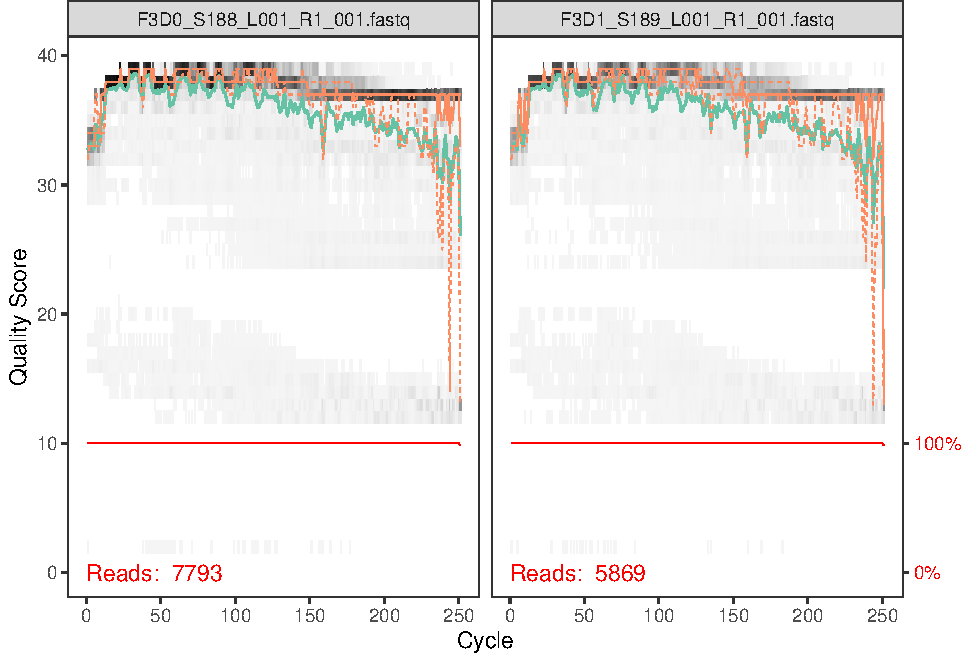
\includegraphics{16sworkshop_files/figure-latex/make_plots-1.pdf}

\begin{Shaded}
\begin{Highlighting}[]
\NormalTok{joint\_fnames}\OtherTok{\textless{}{-}}\FunctionTok{c}\NormalTok{(}\FunctionTok{rbind}\NormalTok{(fnFs,fnRs))}

\FunctionTok{plotQualityProfile}\NormalTok{(joint\_fnames)}
\end{Highlighting}
\end{Shaded}

\begin{verbatim}
## Scale for 'y' is already present. Adding another scale for 'y', which will
## replace the existing scale.
\end{verbatim}

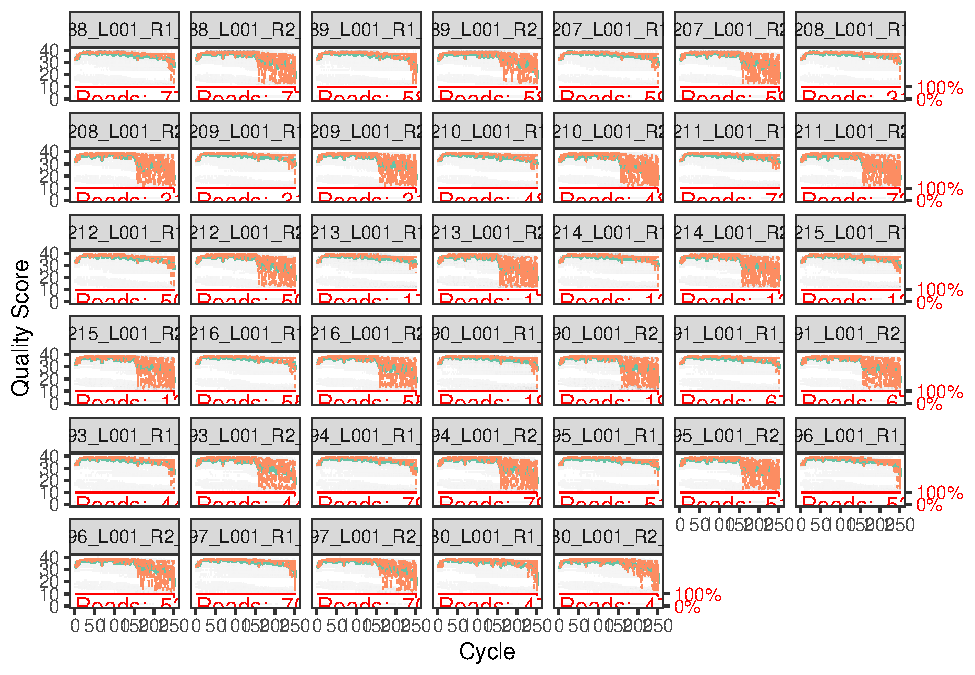
\includegraphics{16sworkshop_files/figure-latex/make_plots-2.pdf}

if there are too many files, use arrangegrob. See here \href{https://cran.r-project.org/web/packages/gridExtra/vignettes/arrangeGrob.html}{here} for details

For the rest of the DADA2 pipelien please \href{https://benjjneb.github.io/dada2/tutorial.html}{visit}

\hypertarget{some-tips}{%
\section{Some tips:}\label{some-tips}}

\begin{enumerate}
\def\labelenumi{\arabic{enumi}.}
\item
  At every step check how many reads are getting filtered. This is very important to make sure that you are not losing too much data.
\item
  If in the filtering step you are losing too many reads, relax the maxEE from 2 to 3 or more. Also check the length that you are truncating at.
\item
  If you are using cutAdapt for quality trimming, you don't have to use truncation in filterandtrim function of DADA2
\item
  Always keep in mind the overlap length for your region of interest. see the figure below for calculation:
\end{enumerate}

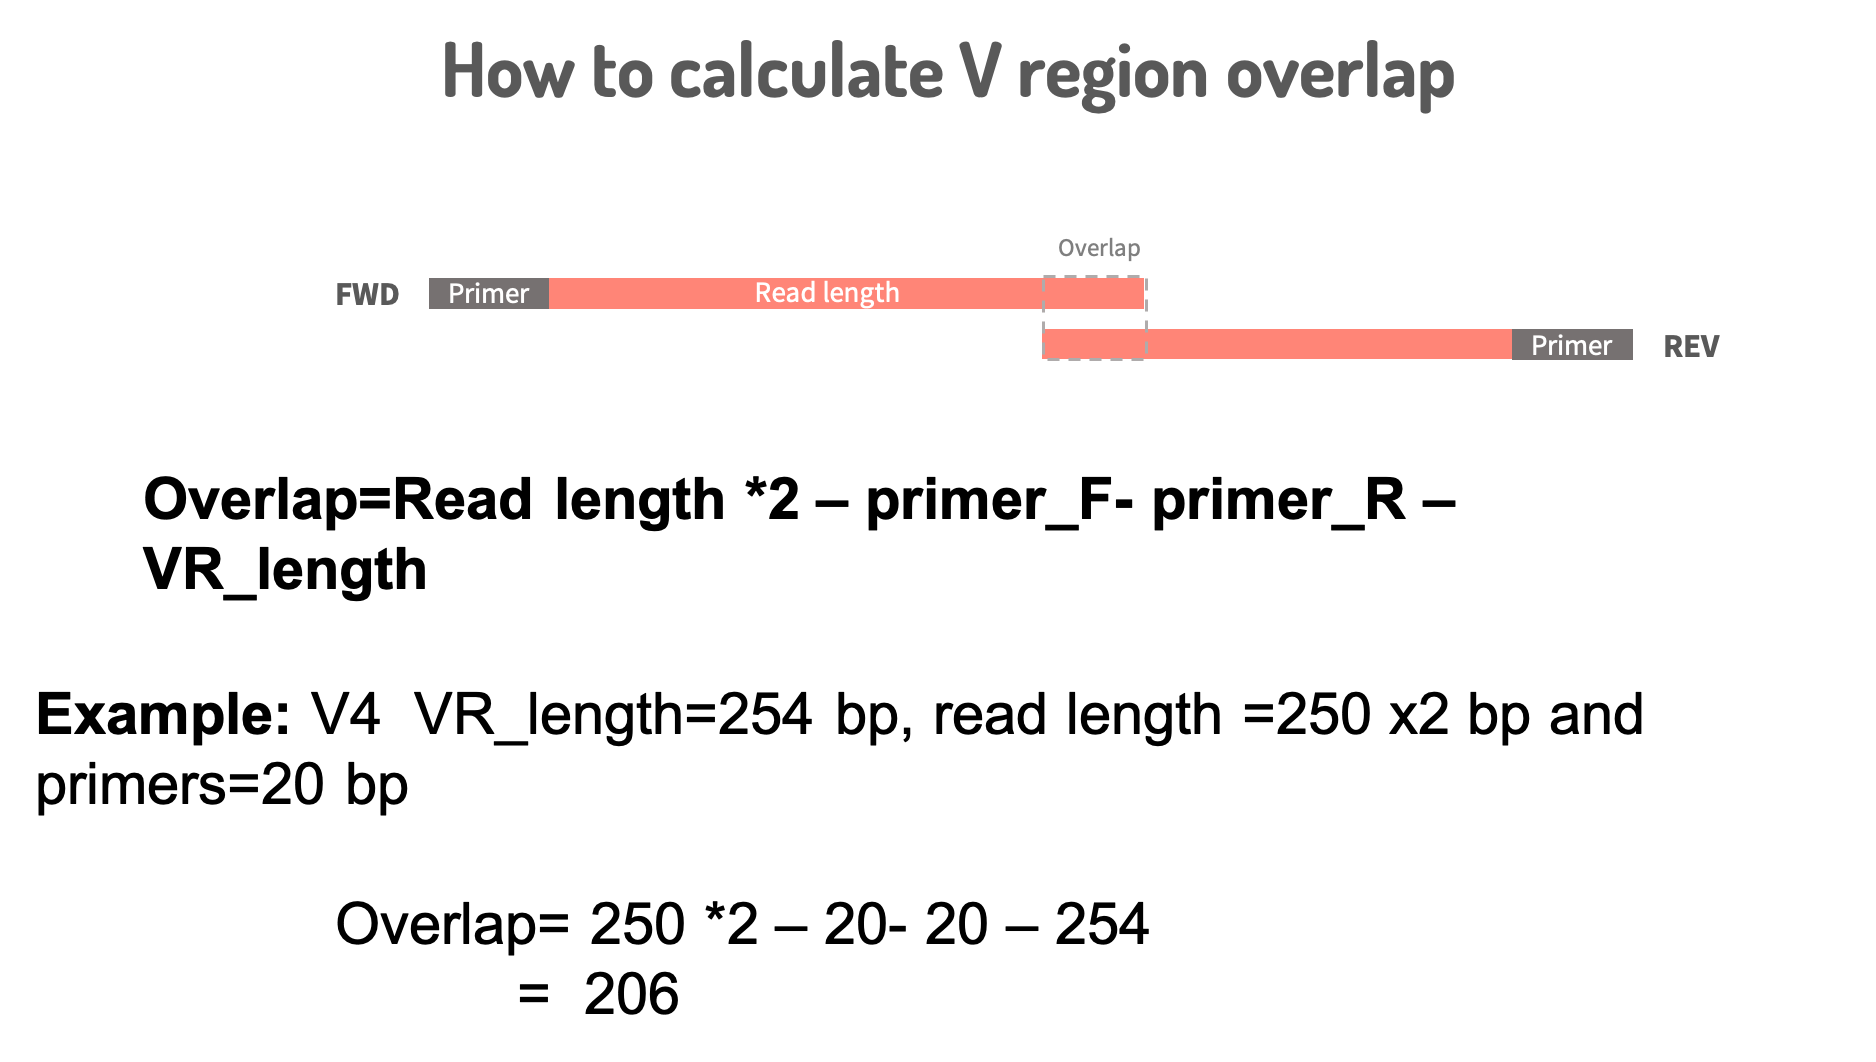
\includegraphics{overlap.png}

\begin{enumerate}
\def\labelenumi{\arabic{enumi}.}
\setcounter{enumi}{4}
\tightlist
\item
  If you lose too many sequences to chimera removal, please check that the primers are removed properly.
\end{enumerate}

\hypertarget{day-two}{%
\chapter{Day Two}\label{day-two}}

\hypertarget{main-concepts-to-be-discussed}{%
\section{Main concepts to be discussed:}\label{main-concepts-to-be-discussed}}

\begin{itemize}
\tightlist
\item
  Finish dada2 pipeline
\item
  Assign Taxonomy
\item
  Intro to Phyolseq package
\item
  Create a Phylum level bar plots
\item
  Alpha diversity plots
\item
  Beta diversity plots
\end{itemize}

Once we are finished using the dada2 package, we will have a sequence table and taxonomy table.

Lets look at the metadata files we have to get more information about these samples.

\begin{Shaded}
\begin{Highlighting}[]
\FunctionTok{library}\NormalTok{(ggplot2)}
\FunctionTok{library}\NormalTok{(dplyr)}
\end{Highlighting}
\end{Shaded}

\begin{verbatim}
## 
## Attaching package: 'dplyr'
\end{verbatim}

\begin{verbatim}
## The following objects are masked from 'package:stats':
## 
##     filter, lag
\end{verbatim}

\begin{verbatim}
## The following objects are masked from 'package:base':
## 
##     intersect, setdiff, setequal, union
\end{verbatim}

\begin{Shaded}
\begin{Highlighting}[]
\NormalTok{time\_info}\OtherTok{\textless{}{-}}\FunctionTok{read.delim}\NormalTok{(}\StringTok{"\textasciitilde{}/projects/16sanalysis\_workshop/workshoptutorial/MiSeq\_SOP/mouse.time.design"}\NormalTok{,}\AttributeTok{sep  =} \StringTok{"}\SpecialCharTok{\textbackslash{}t}\StringTok{"}\NormalTok{)}
\NormalTok{dpw\_info}\OtherTok{\textless{}{-}}\FunctionTok{read.delim}\NormalTok{(}\StringTok{"\textasciitilde{}/projects/16sanalysis\_workshop/workshoptutorial/MiSeq\_SOP/mouse.dpw.metadata"}\NormalTok{,}\AttributeTok{sep  =} \StringTok{"}\SpecialCharTok{\textbackslash{}t}\StringTok{"}\NormalTok{)}

\NormalTok{sample\_info}\OtherTok{\textless{}{-}}\FunctionTok{left\_join}\NormalTok{(time\_info,dpw\_info,}\AttributeTok{by=}\StringTok{"group"}\NormalTok{)}

\FunctionTok{rownames}\NormalTok{(sample\_info)}\OtherTok{\textless{}{-}}\NormalTok{ sample\_info}\SpecialCharTok{$}\NormalTok{group}

\NormalTok{sample\_info}
\end{Highlighting}
\end{Shaded}

\begin{verbatim}
##         group  time dpw
## F3D0     F3D0 Early   0
## F3D1     F3D1 Early   1
## F3D141 F3D141  Late 141
## F3D142 F3D142  Late 142
## F3D143 F3D143  Late 143
## F3D144 F3D144  Late 144
## F3D145 F3D145  Late 145
## F3D146 F3D146  Late 146
## F3D147 F3D147  Late 147
## F3D148 F3D148  Late 148
## F3D149 F3D149  Late 149
## F3D150 F3D150  Late 150
## F3D2     F3D2 Early   2
## F3D3     F3D3 Early   3
## F3D5     F3D5 Early   5
## F3D6     F3D6 Early   6
## F3D7     F3D7 Early   7
## F3D8     F3D8 Early   8
## F3D9     F3D9 Early   9
\end{verbatim}

Lets make a phyloseq object

Now that we have sample\_info lets try to make a phyloseq object out of this

\begin{Shaded}
\begin{Highlighting}[]
\FunctionTok{library}\NormalTok{(phyloseq)}
\NormalTok{taxa}\OtherTok{\textless{}{-}}\FunctionTok{readRDS}\NormalTok{(}\StringTok{"\textasciitilde{}/projects/16sanalysis\_workshop/workshoptutorial/output/taxa.rds"}\NormalTok{)}
\NormalTok{seq}\OtherTok{\textless{}{-}}\FunctionTok{readRDS}\NormalTok{(}\StringTok{"\textasciitilde{}/projects/16sanalysis\_workshop/workshoptutorial/output/seq.rds"}\NormalTok{)}

\NormalTok{ps }\OtherTok{\textless{}{-}} \FunctionTok{phyloseq}\NormalTok{(}\FunctionTok{otu\_table}\NormalTok{(seq,}\AttributeTok{taxa\_are\_rows =}\NormalTok{ F),}
               \FunctionTok{sample\_data}\NormalTok{(sample\_info),}
               \FunctionTok{tax\_table}\NormalTok{(taxa))}

\NormalTok{ps}
\end{Highlighting}
\end{Shaded}

\begin{verbatim}
## phyloseq-class experiment-level object
## otu_table()   OTU Table:         [ 234 taxa and 19 samples ]
## sample_data() Sample Data:       [ 19 samples by 3 sample variables ]
## tax_table()   Taxonomy Table:    [ 234 taxa by 7 taxonomic ranks ]
\end{verbatim}

You can see that this object has an OTU table(ASV table), sample data and tax\_table. You can use functions tax\_table(), sample\_data() and otu\_table() to access the data.

Take a look at:

\begin{itemize}
\tightlist
\item
  subset\_samples()
\item
  subset\_taxa()
\item
  tax\_glom()
\item
  sample\_sums()
\item
  prune\_samples()
\item
  transform\_sample\_counts()
\item
  psmelt()
\end{itemize}

\begin{Shaded}
\begin{Highlighting}[]
\NormalTok{ps2}\OtherTok{\textless{}{-}}\FunctionTok{tax\_glom}\NormalTok{(ps,}\AttributeTok{taxrank =} \StringTok{"Phylum"}\NormalTok{)}
\NormalTok{ps2 }\OtherTok{=} \FunctionTok{transform\_sample\_counts}\NormalTok{(ps2, }\ControlFlowTok{function}\NormalTok{(x) x}\SpecialCharTok{/}\FunctionTok{sum}\NormalTok{(x))}
\NormalTok{pmelt}\OtherTok{\textless{}{-}}\FunctionTok{psmelt}\NormalTok{(ps2) }\SpecialCharTok{\%\textgreater{}\%} \FunctionTok{arrange}\NormalTok{(}\FunctionTok{desc}\NormalTok{(Abundance))}

\NormalTok{cutoff}\OtherTok{\textless{}{-}}\FloatTok{0.005}
\NormalTok{pmelt\_filt}\OtherTok{\textless{}{-}}\NormalTok{pmelt }\SpecialCharTok{\%\textgreater{}\%} \FunctionTok{group\_by}\NormalTok{(Phylum,time) }\SpecialCharTok{\%\textgreater{}\%} \FunctionTok{filter}\NormalTok{(}\FunctionTok{sum}\NormalTok{(Abundance) }\SpecialCharTok{\textgreater{}}\NormalTok{cutoff)}

\FunctionTok{ggplot}\NormalTok{(pmelt\_filt,}\FunctionTok{aes}\NormalTok{(}\AttributeTok{x=}\NormalTok{Sample,}\AttributeTok{y=}\NormalTok{Abundance,}\AttributeTok{color=}\NormalTok{Phylum,}\AttributeTok{fill=}\NormalTok{Phylum)) }\SpecialCharTok{+}\FunctionTok{geom\_bar}\NormalTok{(}\AttributeTok{stat =} \StringTok{"identity"}\NormalTok{)}
\end{Highlighting}
\end{Shaded}

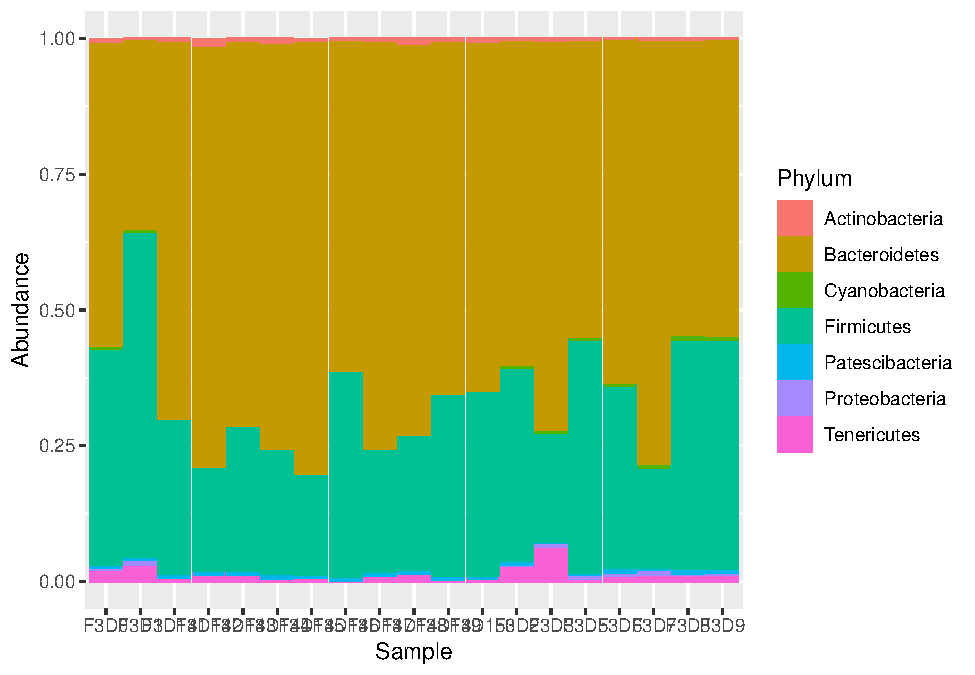
\includegraphics{16sworkshop_files/figure-latex/unnamed-chunk-2-1.pdf}

\begin{Shaded}
\begin{Highlighting}[]
\NormalTok{pmelt\_filt }\SpecialCharTok{\%\textgreater{}\%} \FunctionTok{group\_by}\NormalTok{(time,Phylum) }\SpecialCharTok{\%\textgreater{}\%} \FunctionTok{summarise}\NormalTok{(}\AttributeTok{mean\_Abundance=}\FunctionTok{mean}\NormalTok{(Abundance)) }\SpecialCharTok{\%\textgreater{}\%} \FunctionTok{ggplot}\NormalTok{(.,}\FunctionTok{aes}\NormalTok{(}\AttributeTok{x=}\NormalTok{time,}\AttributeTok{y=}\NormalTok{mean\_Abundance,}\AttributeTok{fill=}\NormalTok{Phylum)) }\SpecialCharTok{+}\FunctionTok{geom\_bar}\NormalTok{(}\AttributeTok{stat=}\StringTok{"identity"}\NormalTok{)}
\end{Highlighting}
\end{Shaded}

\begin{verbatim}
## `summarise()` has grouped output by 'time'. You can override using the `.groups` argument.
\end{verbatim}

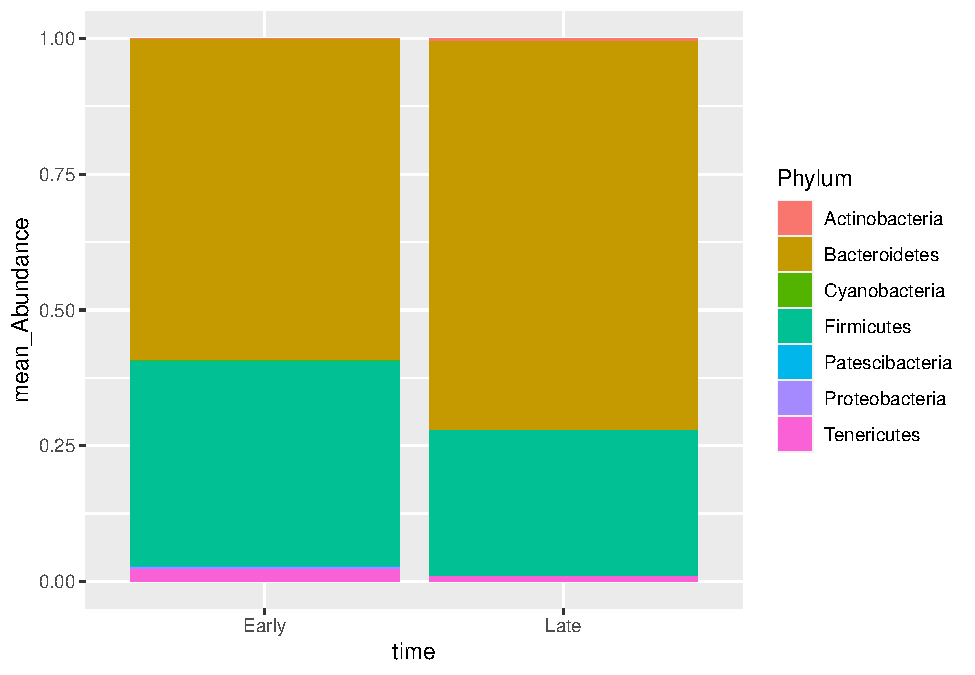
\includegraphics{16sworkshop_files/figure-latex/unnamed-chunk-2-2.pdf}

Figure out how to change the colors to custom colors!!

\begin{Shaded}
\begin{Highlighting}[]
\NormalTok{pmelt\_filt }\SpecialCharTok{\%\textgreater{}\%} \FunctionTok{group\_by}\NormalTok{(time,Phylum) }\SpecialCharTok{\%\textgreater{}\%} \FunctionTok{summarise}\NormalTok{(}\AttributeTok{mean=}\FunctionTok{mean}\NormalTok{(Abundance))}
\end{Highlighting}
\end{Shaded}

\begin{verbatim}
## `summarise()` has grouped output by 'time'. You can override using the `.groups` argument.
\end{verbatim}

\begin{verbatim}
## # A tibble: 12 x 3
## # Groups:   time [2]
##    time  Phylum              mean
##    <fct> <fct>              <dbl>
##  1 Early Actinobacteria  0.00133 
##  2 Early Bacteroidetes   0.592   
##  3 Early Cyanobacteria   0.000594
##  4 Early Firmicutes      0.378   
##  5 Early Patescibacteria 0.00285 
##  6 Early Proteobacteria  0.00331 
##  7 Early Tenericutes     0.0218  
##  8 Late  Actinobacteria  0.00472 
##  9 Late  Bacteroidetes   0.716   
## 10 Late  Firmicutes      0.269   
## 11 Late  Patescibacteria 0.000993
## 12 Late  Tenericutes     0.00845
\end{verbatim}

\hypertarget{alpha-beta-diversity}{%
\section{Alpha \& beta Diversity}\label{alpha-beta-diversity}}

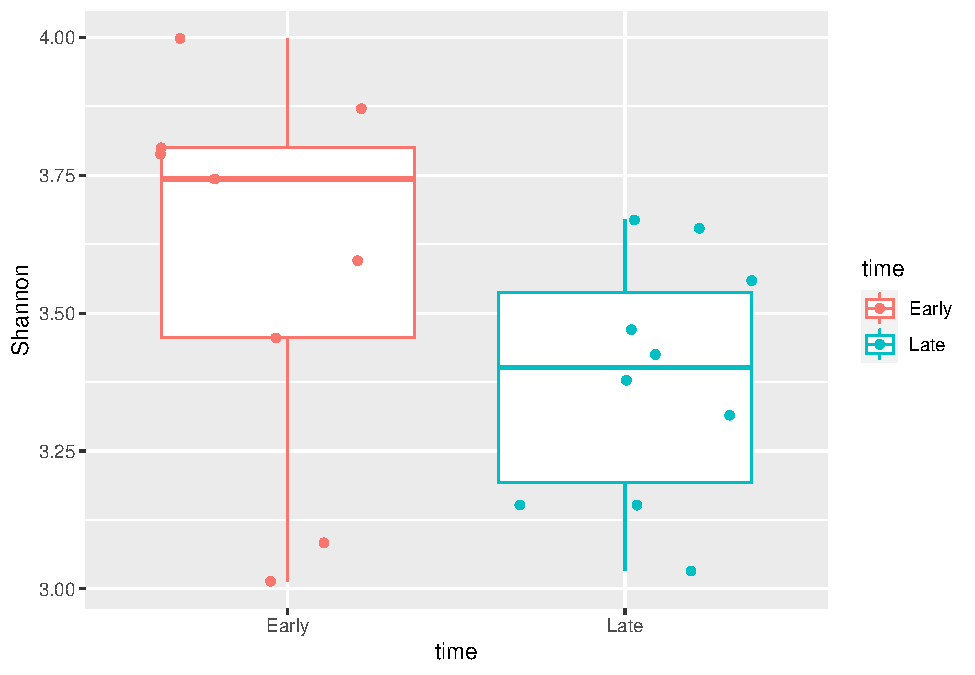
\includegraphics{16sworkshop_files/figure-latex/alpha diversit-1.pdf}

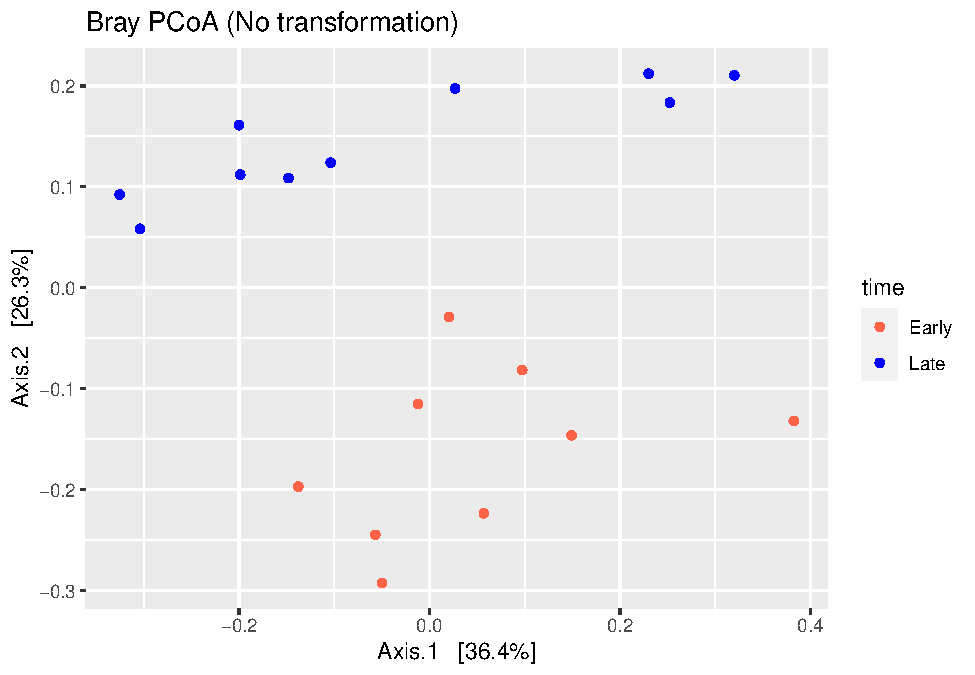
\includegraphics{16sworkshop_files/figure-latex/unnamed-chunk-3-1.pdf} 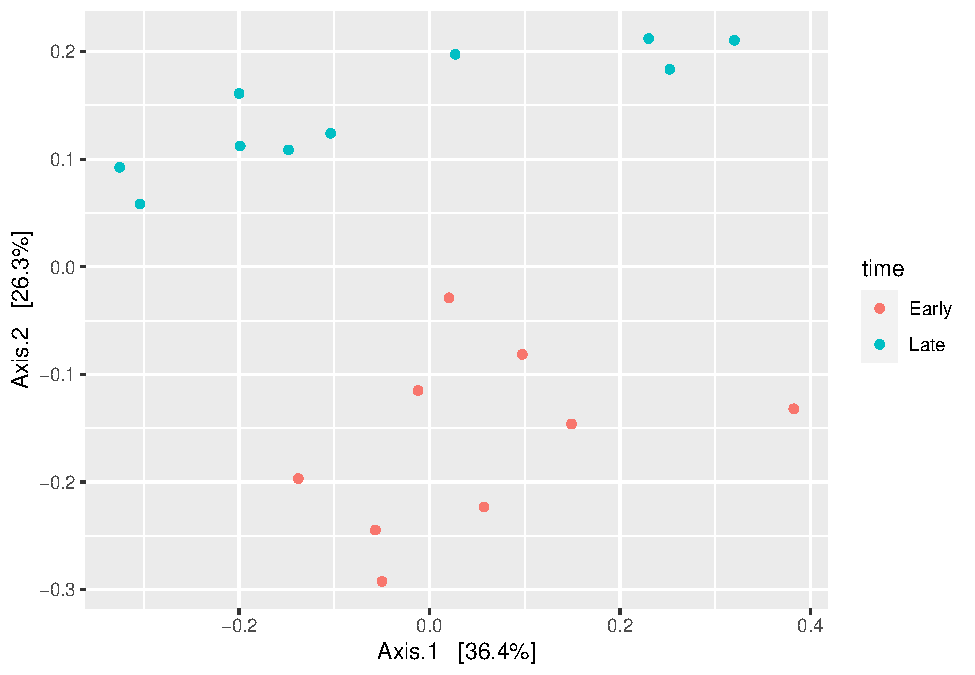
\includegraphics{16sworkshop_files/figure-latex/unnamed-chunk-3-2.pdf}

\hypertarget{project}{%
\chapter{Project}\label{project}}

\hypertarget{setup}{%
\section{Setup}\label{setup}}

Please download the raw data \href{https://www.dropbox.com/sh/1oy9upgzxlsra9y/AAANkbCj36lvP6vEQucE7fYna?dl=0}{here}.

These samples are from a study looking at the effect of a prebiotic on the gut microbiota of children with type 1 diabetes. To invesigate this, the researchers took samples at three timepoints (baseline, 3 months, and 6 months) and sequenced the \textbf{V3-V4} region of the 16S rRNA gene.

\hypertarget{task-1-ignore-this-task}{%
\section{Task 1 (Ignore this task)}\label{task-1-ignore-this-task}}

The first step with all sequence data is to ensure the primers have been removed. The two most common tools to accomplish this are \textbf{Cutadapt} and \textbf{Trimmomatic}.

Note: both of these tools can be used for quality trimming as well as primer removal but here we will perform the quality trimming in dada2 instead.

\hypertarget{cutadapt-1}{%
\subsection{Cutadapt}\label{cutadapt-1}}

You can find the documentation for this tool \href{https://cutadapt.readthedocs.io/en/stable/}{here}.

These are the parameters that contain the primer sequences:

\begin{itemize}
\tightlist
\item
  \texttt{-g\ :\ forward\ primer}
\item
  \texttt{-G\ :\ reverse\ primer}
\item
  \texttt{-a\ :\ reverse\ primer,\ reverse\ complement}
\item
  \texttt{-A\ :\ forward\ primer,\ reverse\ complement}
\end{itemize}

For this dataset, these are the appropriate primers:

\begin{verbatim}
-g TCGTCGGCAGCGTCAGATGTGTATAAGAGACAGCCTACGGGNGGCWGCAG
-G GTCTCGTGGGCTCGGAGATGTGTATAAGAGACAGGACTACHVGGGTATCTAATCC
-a GGATTAGATACCCBDGTAGTCCTGTCTCTTATACACATCTCCGAGCCCACGAGAC
-A CTGCWGCCNCCCGTAGGCTGTCTCTTATACACATCTGACGCTGCCGACGA
\end{verbatim}

Here is an example of how to execute Cutadapt from the command line:

\begin{verbatim}
cutadapt -g <sequence> -G <sequence> -a <sequence> -A <sequence> -o output_forward.fastq -p output_reverse.fastq input_forward.fastq input_reverse.fastq
\end{verbatim}

Note that you can also run cutadapt from within R. You can find instructions on how to do that \href{https://benjjneb.github.io/dada2/ITS_workflow.html}{here}.

\hypertarget{trimmomatic}{%
\subsection{Trimmomatic}\label{trimmomatic}}

You can find the documentation for this tool \href{http://www.usadellab.org/cms/?page=trimmomatic}{here}.

Instead of specifying forward and reverse reads, Trimmomatic takes a fasta file as input and searches the reads for all sequences in the files. When using Trimmomatic on paired-end reads, you will get four output files: forward and reverse reads that are still paired (reads for which both forward and reverse were kept) and forward and reverse reads that are unpaired. In general, the number of unpaired reads should be small and you can continue with your analysis without these.

For this dataset, you can use \href{https://www.dropbox.com/s/wc2kihxfep23ycw/v3v4primers.fa?dl=0}{this fasta}.

Here is an example of how to execute Trimmomatic from the command line:

\begin{verbatim}
trimmomatic PE input_forward.fq.gz input_reverse.fq.gz output_forward_paired.fq.gz output_forward_unpaired.fq.gz output_reverse_paired.fq.gz output_reverse_unpaired.fq.gz ILLUMINACLIP:v3v4primers.fa:2:30:10:2:keepBothReads LEADING:0 TRAILING:0 MINLEN:0
\end{verbatim}

\hypertarget{primers-removed}{%
\subsection{Primers removed}\label{primers-removed}}

If you don't care about using either of these tools and want to move on to the next step, you can find the sequences with the primers removed \href{https://www.dropbox.com/s/qrf24anx9zllp9t/trimmed_data.zip?dl=0}{here}.

\hypertarget{task-2}{%
\section{Task 2}\label{task-2}}

Use the dada2 pipeline to generate a table of ASVs and a taxonomy table.

\begin{enumerate}
\def\labelenumi{\arabic{enumi}.}
\tightlist
\item
  Plot quality profiles of the reads for all samples. Save these as pdf files.
\item
  Try a couple of sets of filtering params and determine the best choice.
\item
  Filter and trim the data and generate the quality plots again. Save these as well.
\item
  Learn the error rates and visually inspect the estimated error rates.
\item
  Infer samples.
\item
  Merge paired reads.
\item
  Construct sequence table.
\item
  Remove chimeras.
\item
  Track reads through the pipeline and ensure that no step of the analysis removed a large/unreasonable proportion of the reads.
\item
  Assign taxonomy using the Silva databse.
\item
  Save the ASV table and taxonomy table using the \texttt{saveRDS()} function.
\end{enumerate}

\hypertarget{task-3}{%
\section{Task 3}\label{task-3}}

Use the phyloseq package to generate do some basic analysis. For this section you will need the project metadata files that you already downloaded

\begin{enumerate}
\def\labelenumi{\arabic{enumi}.}
\tightlist
\item
  Generate a histogram of the number of reads per sample. Does this look okay?
\item
  Generate a table of alpha diversity measures (Shannon, Simspon, and Chao1) and use this table to plot alpha diversity by treatment and timepoint.
\item
  Transform the data to relative abundances and remove ASVs that are only present in less than 5\% of the samples.
\item
  Perform a principal component analysis (PCoA) using the \texttt{ordinate()} function and \texttt{distance\ =\ "bray"}. Plot beta diversity.
\item
  Explore the composition of each sample by generating bar plots of the relative abundances at the level of phylum, family, and genus. For family and genus, plot only the top 10 most abundant taxa.
\end{enumerate}

\hypertarget{project-solutions}{%
\section{Project solutions}\label{project-solutions}}

\hypertarget{task-2---dada2}{%
\subsection{Task 2 - dada2}\label{task-2---dada2}}

For this section, the solution closely resembles the code from the \href{http://benjjneb.github.io/dada2/tutorial.html}{dada2 tutorial}. The main challenge is to determine the appropriate filtering parameters.

Here are the quality profiles for the forward and reverse reads for samples 01MP-1 and 03KW-1. You can see that the quality of the ends of the reverse reads are much worse than the forward reads.

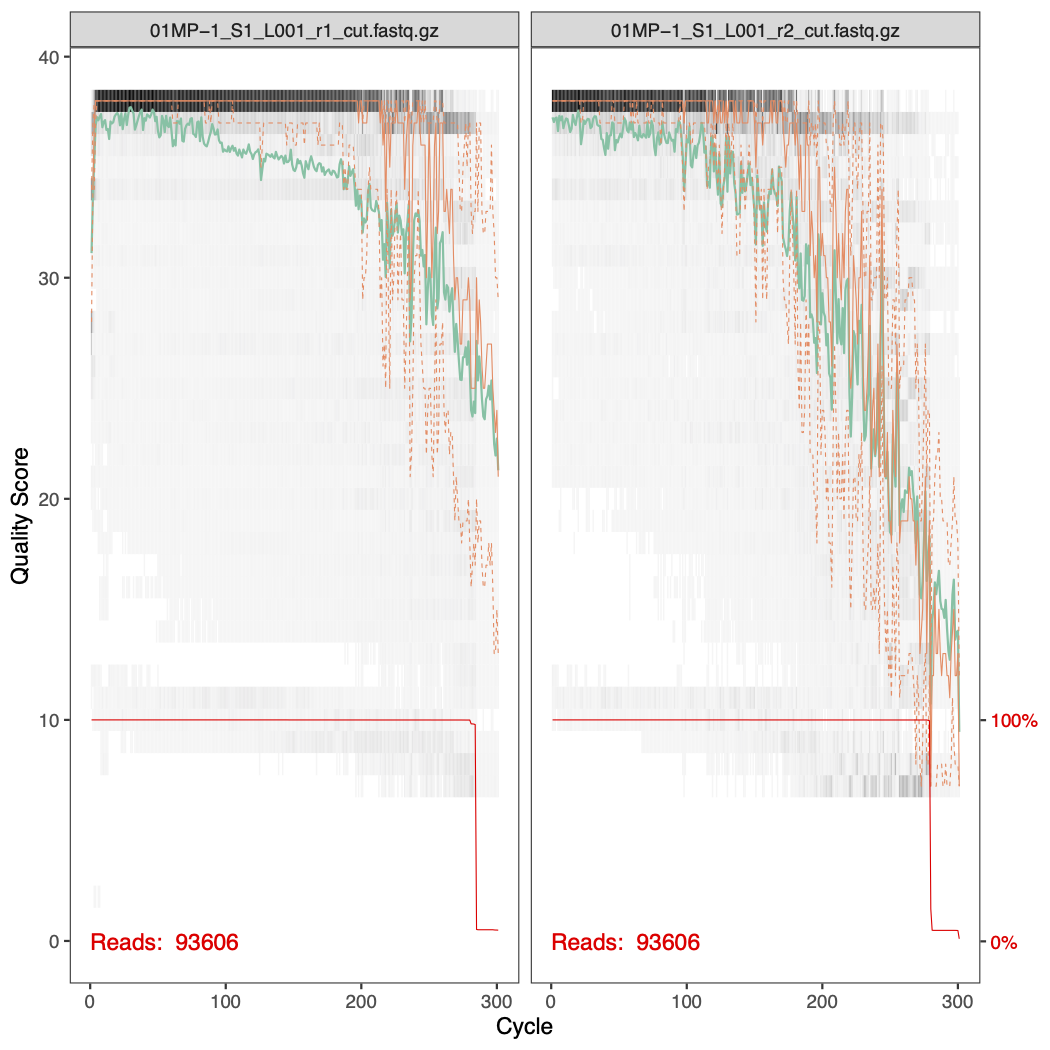
\includegraphics{book/project_files/quality_01MP-1.png}

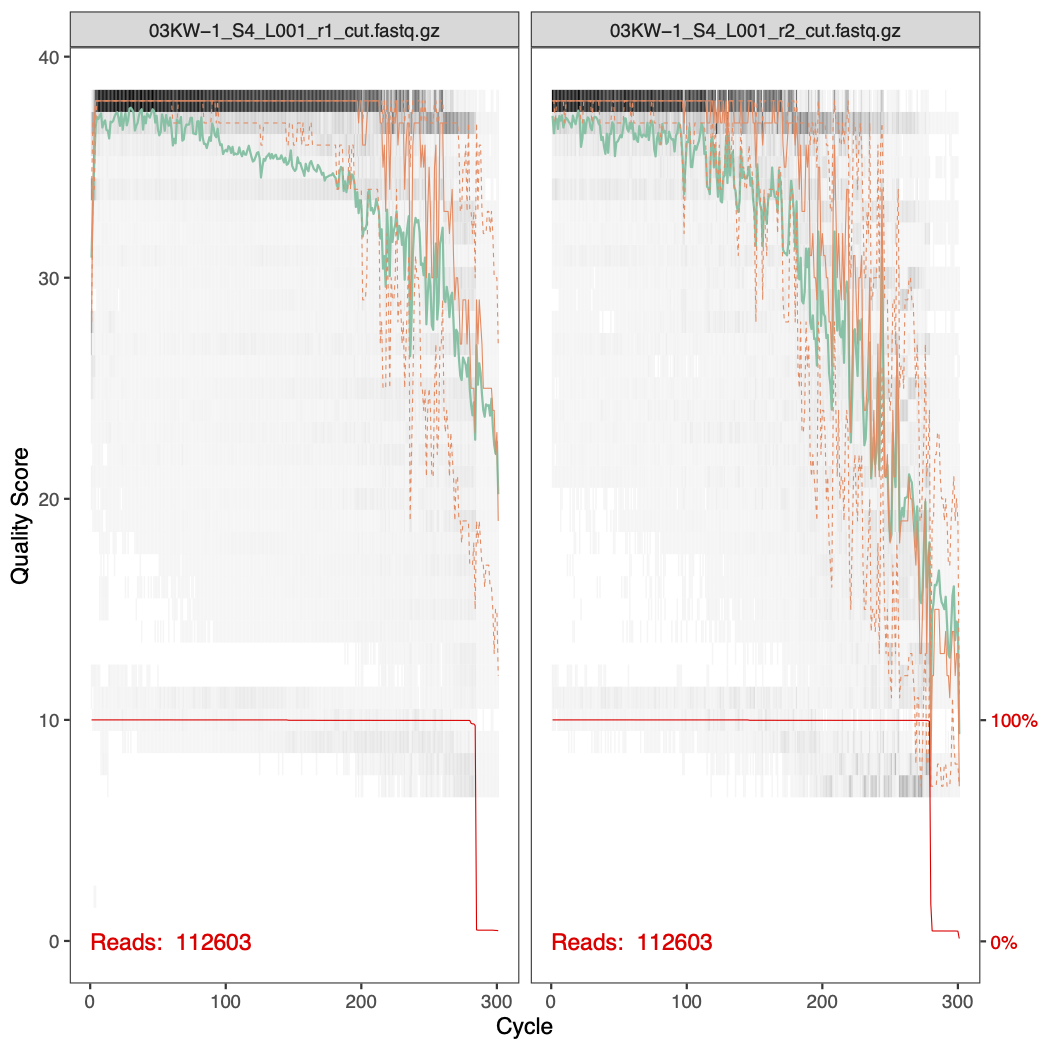
\includegraphics{book/project_files/quality_03KW-1.png}
To help guide our parameter choice, here is a plot showing the percentage of reads that passed filtering as a produce of changing both the forward error rate and the reverse error rate.

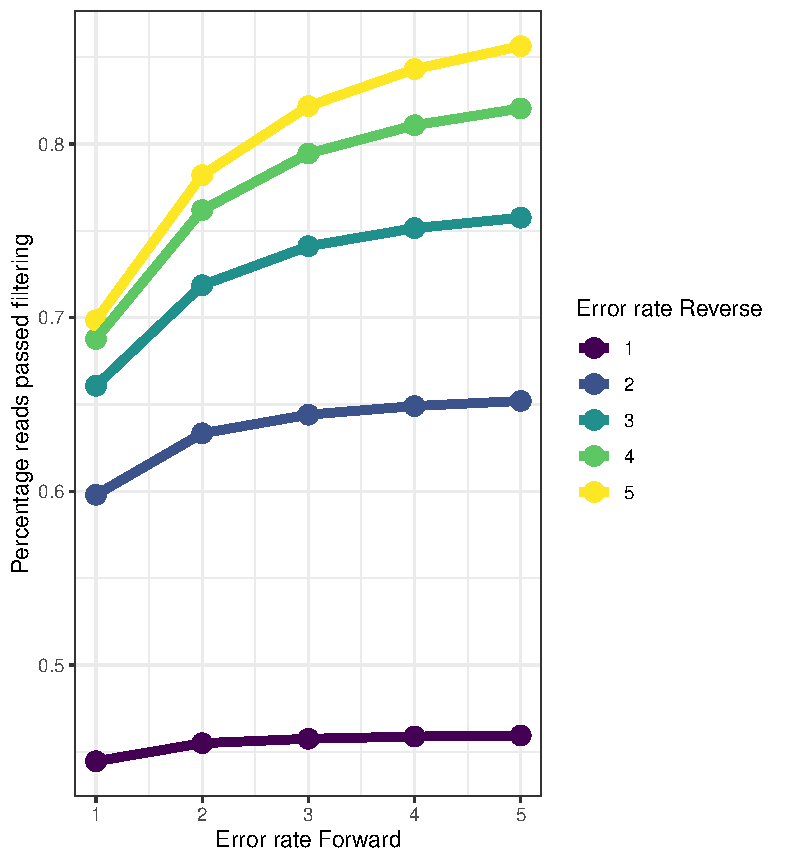
\includegraphics[width=10.93in]{book/project_files/filt_params}

Based on this, we should choose an error rate of \texttt{c(3,4)} or something similar. Note that the truncation length used here was \texttt{c(265,245)}.

After filtering, we look the effect of the filtering on the quality profiles. Below are the before and after filtering quality profiles of the forward and reverse reads of sample 01MP-1.

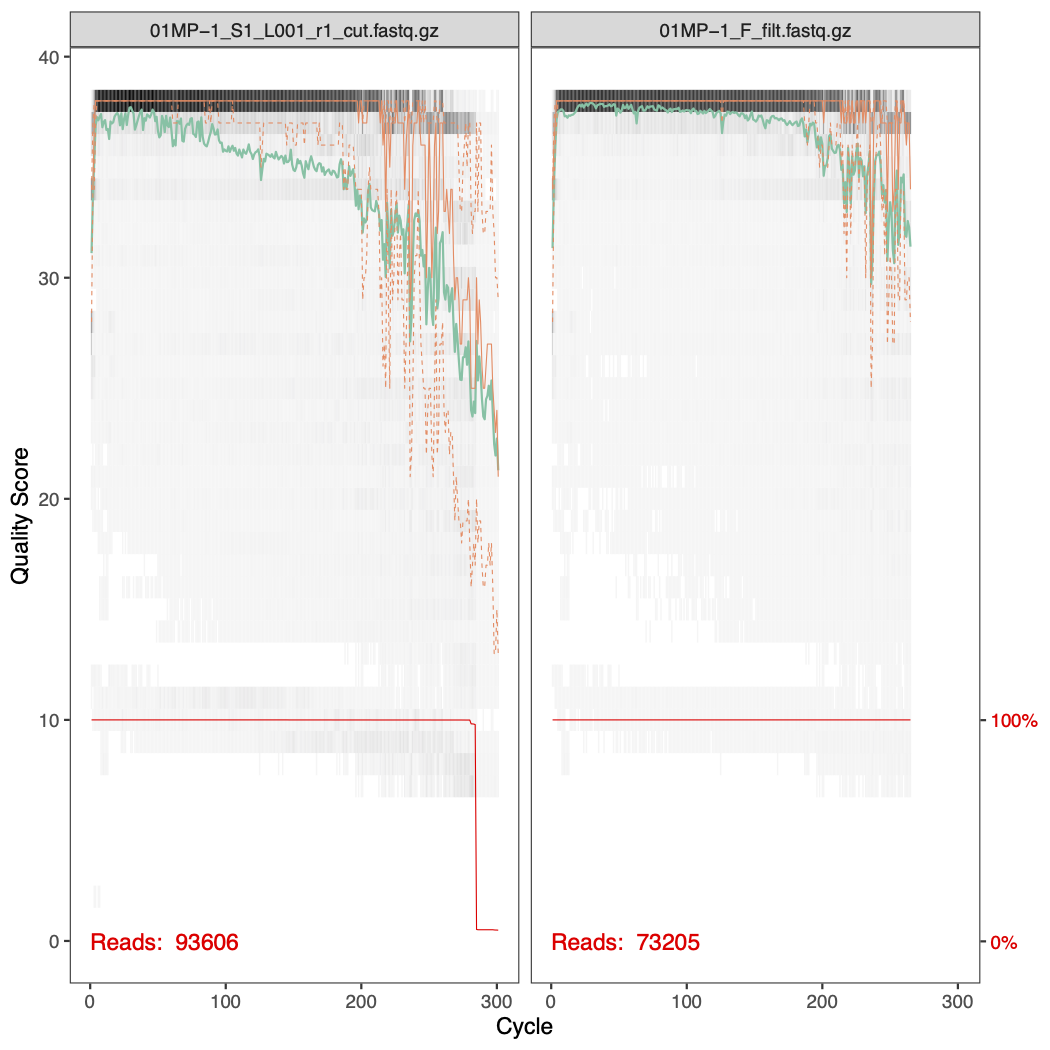
\includegraphics{book/project_files/quality_filt_for_01MP-1.png}

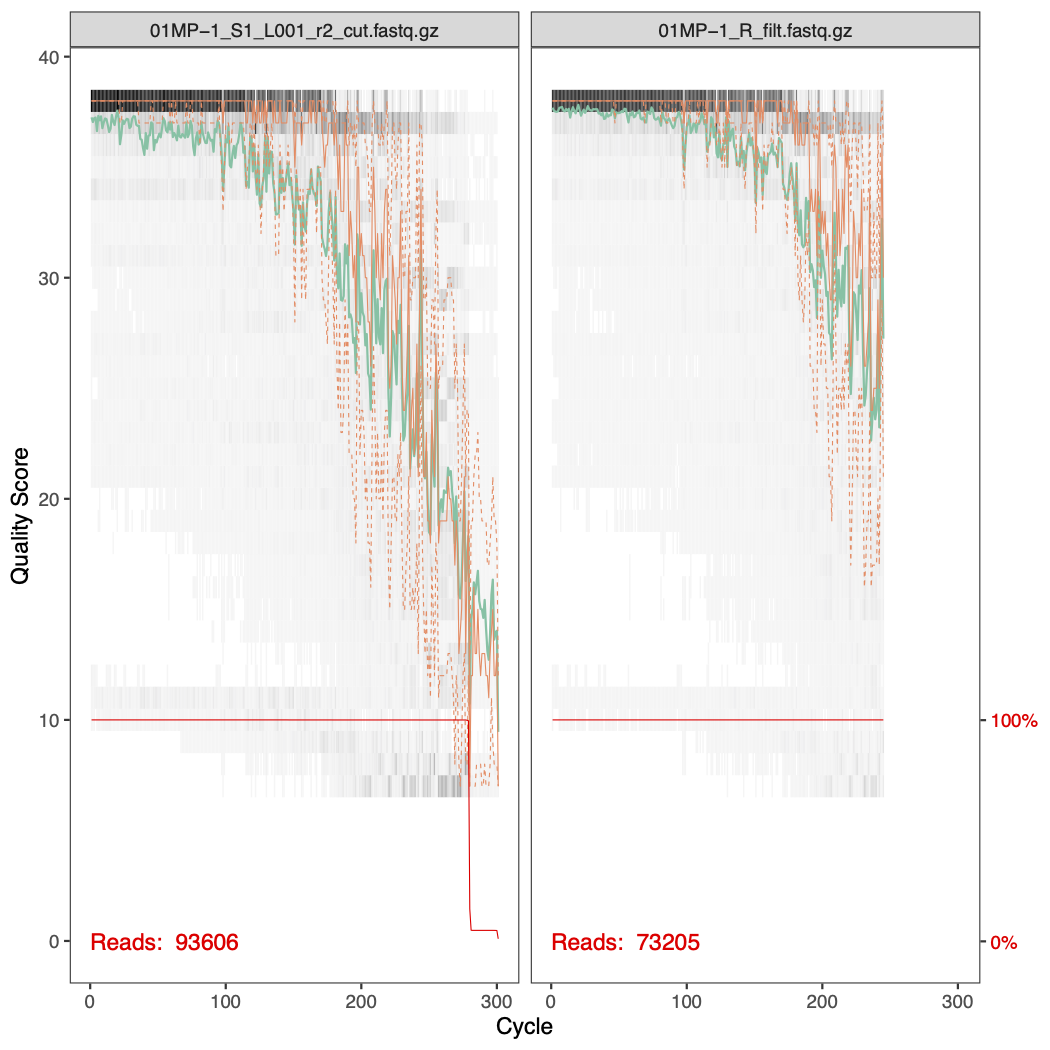
\includegraphics{book/project_files/quality_filt_rev_01MP-1.png}

\hypertarget{task-3---phyloseq}{%
\subsection{Task 3 - phyloseq}\label{task-3---phyloseq}}

Following the dada2 pipeline, we will have a sequence table and a taxonomy table.

\begin{Shaded}
\begin{Highlighting}[]
\NormalTok{path }\OtherTok{\textless{}{-}} \StringTok{"./book/project\_files/"}

\CommentTok{\# Read in files}
\NormalTok{seqtab }\OtherTok{\textless{}{-}} \FunctionTok{readRDS}\NormalTok{(}\FunctionTok{file.path}\NormalTok{(path, }\StringTok{"seqtab.rds"}\NormalTok{))}
\NormalTok{taxa }\OtherTok{\textless{}{-}} \FunctionTok{readRDS}\NormalTok{(}\FunctionTok{file.path}\NormalTok{(path, }\StringTok{"taxa.rds"}\NormalTok{))}
\NormalTok{info }\OtherTok{\textless{}{-}} \FunctionTok{read.table}\NormalTok{(}\FunctionTok{file.path}\NormalTok{(path, }\StringTok{"project\_metadata.txt"}\NormalTok{), }\AttributeTok{header =} \ConstantTok{TRUE}\NormalTok{)}

\CommentTok{\# Match sample names}
\FunctionTok{rownames}\NormalTok{(info) }\OtherTok{\textless{}{-}} \FunctionTok{rownames}\NormalTok{(seqtab)}

\CommentTok{\# Make a phyloseq object}
\NormalTok{ps }\OtherTok{\textless{}{-}} \FunctionTok{phyloseq}\NormalTok{(}\FunctionTok{otu\_table}\NormalTok{(seqtab, }\AttributeTok{taxa\_are\_rows=}\ConstantTok{FALSE}\NormalTok{), }\FunctionTok{sample\_data}\NormalTok{(info), }\FunctionTok{tax\_table}\NormalTok{(taxa))}

\CommentTok{\# Make timepoint a factor}
\FunctionTok{sample\_data}\NormalTok{(ps)}\SpecialCharTok{$}\NormalTok{timepoint }\OtherTok{\textless{}{-}} \FunctionTok{as.factor}\NormalTok{(}\FunctionTok{sample\_data}\NormalTok{(ps)}\SpecialCharTok{$}\NormalTok{timepoint)}

\DocumentationTok{\#\# Histogram of reads per sample}
\NormalTok{sums }\OtherTok{\textless{}{-}} \FunctionTok{rowSums}\NormalTok{(}\FunctionTok{otu\_table}\NormalTok{(ps))}
\NormalTok{counts }\OtherTok{\textless{}{-}} \FunctionTok{data.frame}\NormalTok{(}\FunctionTok{as}\NormalTok{(}\FunctionTok{sample\_data}\NormalTok{(ps), }\StringTok{"data.frame"}\NormalTok{), }\AttributeTok{totalreads =}\NormalTok{ sums)}

\NormalTok{qq }\OtherTok{\textless{}{-}} \FunctionTok{ggplot}\NormalTok{(counts, }\FunctionTok{aes}\NormalTok{(totalreads)) }\SpecialCharTok{+} \FunctionTok{geom\_histogram}\NormalTok{(}\AttributeTok{binwidth =} \FloatTok{0.02}\NormalTok{) }\SpecialCharTok{+} \FunctionTok{ggtitle}\NormalTok{(}\StringTok{"Read counts per sample"}\NormalTok{) }\SpecialCharTok{+} \FunctionTok{scale\_x\_log10}\NormalTok{()}
\NormalTok{qq}
\end{Highlighting}
\end{Shaded}

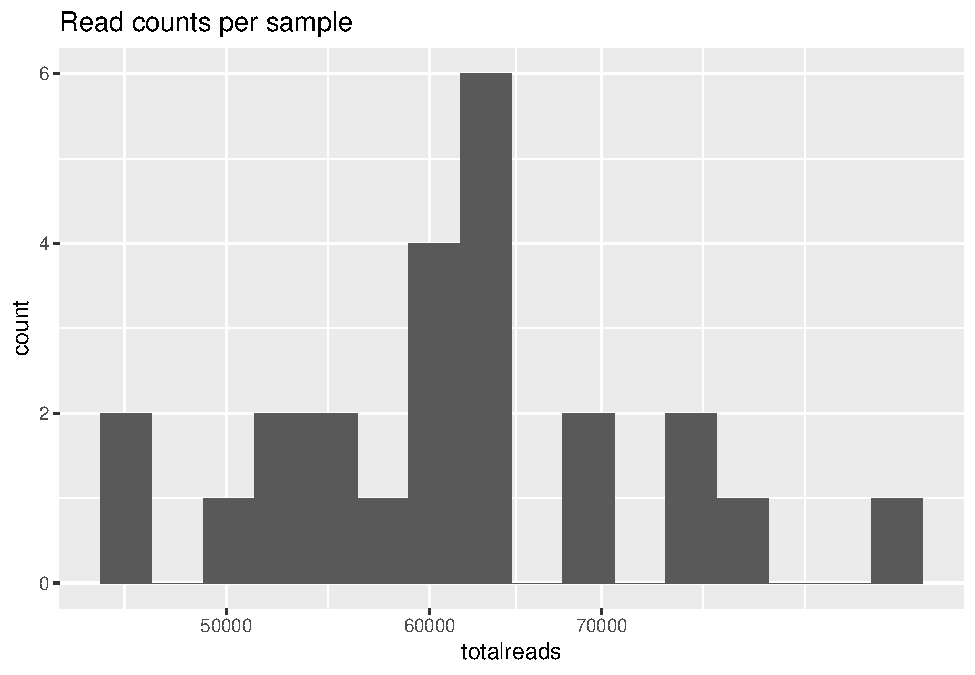
\includegraphics{16sworkshop_files/figure-latex/unnamed-chunk-6-1.pdf}

\begin{Shaded}
\begin{Highlighting}[]
\DocumentationTok{\#\# Alpha diversity}

\DocumentationTok{\#\# Make table of alpha diversity calculations}
\NormalTok{alpha }\OtherTok{\textless{}{-}} \FunctionTok{estimate\_richness}\NormalTok{(ps, }\AttributeTok{measures =} \FunctionTok{c}\NormalTok{(}\StringTok{"Chao1"}\NormalTok{, }\StringTok{"Shannon"}\NormalTok{, }\StringTok{"Simpson"}\NormalTok{))}
\NormalTok{alpha\_info }\OtherTok{\textless{}{-}} \FunctionTok{sample\_data}\NormalTok{(ps)}
\NormalTok{aa }\OtherTok{\textless{}{-}} \FunctionTok{cbind}\NormalTok{(alpha, alpha\_info)}


\NormalTok{a0 }\OtherTok{\textless{}{-}} \FunctionTok{ggplot}\NormalTok{(aa, }\FunctionTok{aes}\NormalTok{(}\AttributeTok{x =}\NormalTok{ treatment, }\AttributeTok{y =}\NormalTok{ Shannon, }\AttributeTok{fill =}\NormalTok{ timepoint)) }\SpecialCharTok{+}
  \FunctionTok{geom\_boxplot}\NormalTok{(}\AttributeTok{outlier.fill =} \ConstantTok{NULL}\NormalTok{, }\AttributeTok{outlier.shape =} \DecValTok{21}\NormalTok{) }\SpecialCharTok{+}
  \FunctionTok{theme\_bw}\NormalTok{() }\SpecialCharTok{+}
  \FunctionTok{geom\_point}\NormalTok{(}\AttributeTok{position =} \FunctionTok{position\_dodge}\NormalTok{(}\AttributeTok{width =} \FloatTok{0.75}\NormalTok{))}
\NormalTok{a0}
\end{Highlighting}
\end{Shaded}

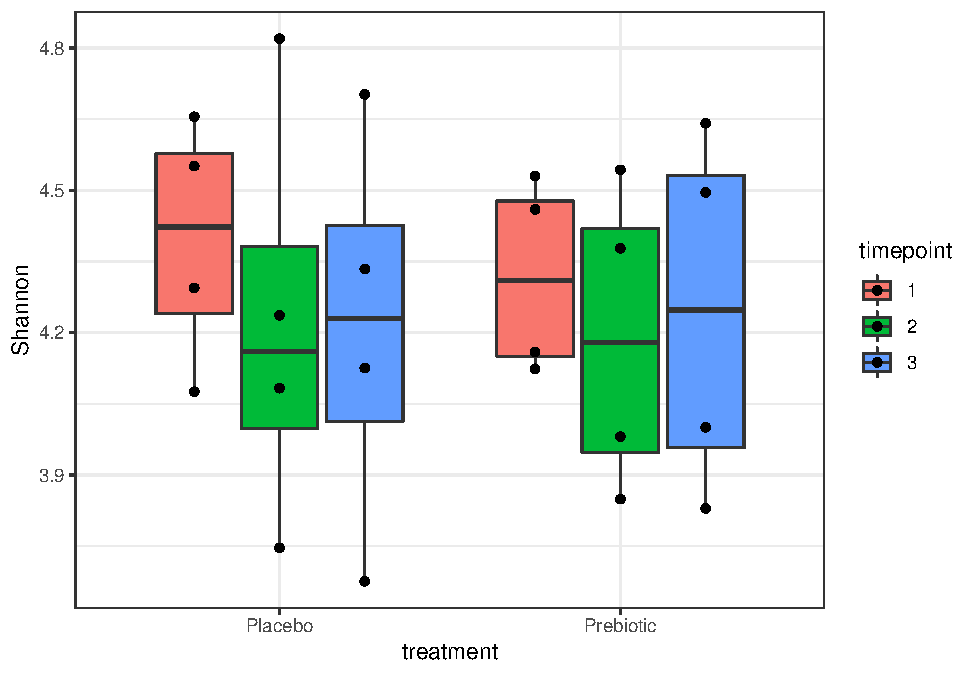
\includegraphics{16sworkshop_files/figure-latex/unnamed-chunk-6-2.pdf}

\begin{Shaded}
\begin{Highlighting}[]
\DocumentationTok{\#\# Beta diversity}

\CommentTok{\# transform to relative abundace}
\NormalTok{rel }\OtherTok{\textless{}{-}} \FunctionTok{transform\_sample\_counts}\NormalTok{(ps, }\ControlFlowTok{function}\NormalTok{(x) x }\SpecialCharTok{/} \FunctionTok{sum}\NormalTok{(x))}
\CommentTok{\# filter out low prevalence ASVs}
\NormalTok{prevdf }\OtherTok{\textless{}{-}} \FunctionTok{apply}\NormalTok{(}\AttributeTok{X =} \FunctionTok{otu\_table}\NormalTok{(ps), }\AttributeTok{MARGIN =} \FunctionTok{ifelse}\NormalTok{(}\FunctionTok{taxa\_are\_rows}\NormalTok{(ps), }\AttributeTok{yes =} \DecValTok{1}\NormalTok{, }\AttributeTok{no =} \DecValTok{2}\NormalTok{), }\AttributeTok{FUN =} \ControlFlowTok{function}\NormalTok{(x)\{}\FunctionTok{sum}\NormalTok{(x }\SpecialCharTok{\textgreater{}} \DecValTok{0}\NormalTok{)\})}
\NormalTok{prevdf }\OtherTok{\textless{}{-}} \FunctionTok{data.frame}\NormalTok{(}\AttributeTok{prevalence =}\NormalTok{ prevdf, }\AttributeTok{total\_abundance =} \FunctionTok{taxa\_sums}\NormalTok{(ps), }\FunctionTok{tax\_table}\NormalTok{(ps))}
\NormalTok{prevalence\_threshold }\OtherTok{\textless{}{-}} \FloatTok{0.05} \SpecialCharTok{*} \FunctionTok{nsamples}\NormalTok{(ps)}
\NormalTok{keeptaxa }\OtherTok{\textless{}{-}} \FunctionTok{rownames}\NormalTok{(prevdf)[prevdf}\SpecialCharTok{$}\NormalTok{prevalence }\SpecialCharTok{\textgreater{}=}\NormalTok{ prevalence\_threshold]}
\NormalTok{relf }\OtherTok{\textless{}{-}} \FunctionTok{prune\_taxa}\NormalTok{(keeptaxa, rel)}
\NormalTok{psf }\OtherTok{\textless{}{-}} \FunctionTok{prune\_taxa}\NormalTok{(keeptaxa, ps)}

\NormalTok{ord }\OtherTok{\textless{}{-}} \FunctionTok{ordinate}\NormalTok{(relf, }\AttributeTok{method =} \StringTok{"PCoA"}\NormalTok{, }\AttributeTok{distance =} \StringTok{"bray"}\NormalTok{)}
\NormalTok{b0 }\OtherTok{\textless{}{-}} \FunctionTok{plot\_ordination}\NormalTok{(relf, ord, }\AttributeTok{shape =} \StringTok{"treatment"}\NormalTok{, }\AttributeTok{color =} \StringTok{"timepoint"}\NormalTok{) }\SpecialCharTok{+}
  \FunctionTok{theme\_bw}\NormalTok{()}
\NormalTok{b0}
\end{Highlighting}
\end{Shaded}

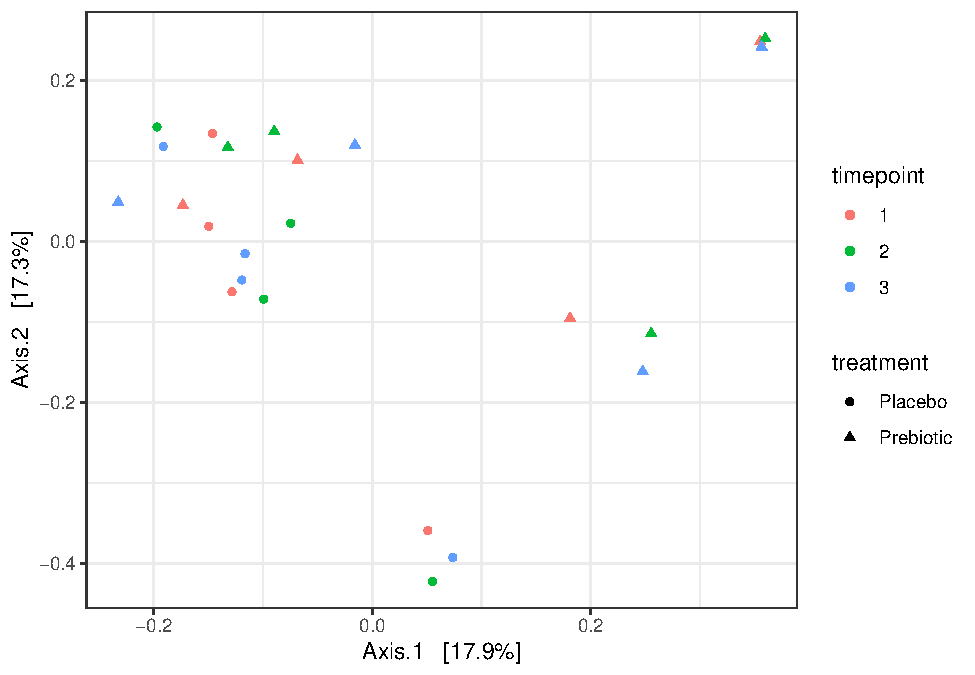
\includegraphics{16sworkshop_files/figure-latex/unnamed-chunk-6-3.pdf}

\begin{Shaded}
\begin{Highlighting}[]
\DocumentationTok{\#\# Composition}

\CommentTok{\# Agglomerate to phylum, family, and genus level}
\NormalTok{phy }\OtherTok{\textless{}{-}} \FunctionTok{tax\_glom}\NormalTok{(relf, }\StringTok{"Phylum"}\NormalTok{)}
\NormalTok{fam }\OtherTok{\textless{}{-}} \FunctionTok{tax\_glom}\NormalTok{(relf, }\StringTok{"Family"}\NormalTok{)}
\NormalTok{gen }\OtherTok{\textless{}{-}} \FunctionTok{tax\_glom}\NormalTok{(relf, }\StringTok{"Genus"}\NormalTok{)}

\NormalTok{phymelt }\OtherTok{\textless{}{-}} \FunctionTok{psmelt}\NormalTok{(phy)}
\NormalTok{c0 }\OtherTok{\textless{}{-}} \FunctionTok{ggplot}\NormalTok{(phymelt, }\FunctionTok{aes}\NormalTok{(sample\_id, Abundance, }\AttributeTok{fill =}\NormalTok{ Phylum)) }\SpecialCharTok{+}
  \FunctionTok{geom\_bar}\NormalTok{(}\AttributeTok{stat =} \StringTok{"identity"}\NormalTok{) }\SpecialCharTok{+}
  \FunctionTok{theme\_bw}\NormalTok{() }\SpecialCharTok{+}
  \FunctionTok{facet\_wrap}\NormalTok{(}\SpecialCharTok{\textasciitilde{}}\NormalTok{treatment, }\AttributeTok{scales =} \StringTok{"free\_x"}\NormalTok{)}
\NormalTok{c0}
\end{Highlighting}
\end{Shaded}

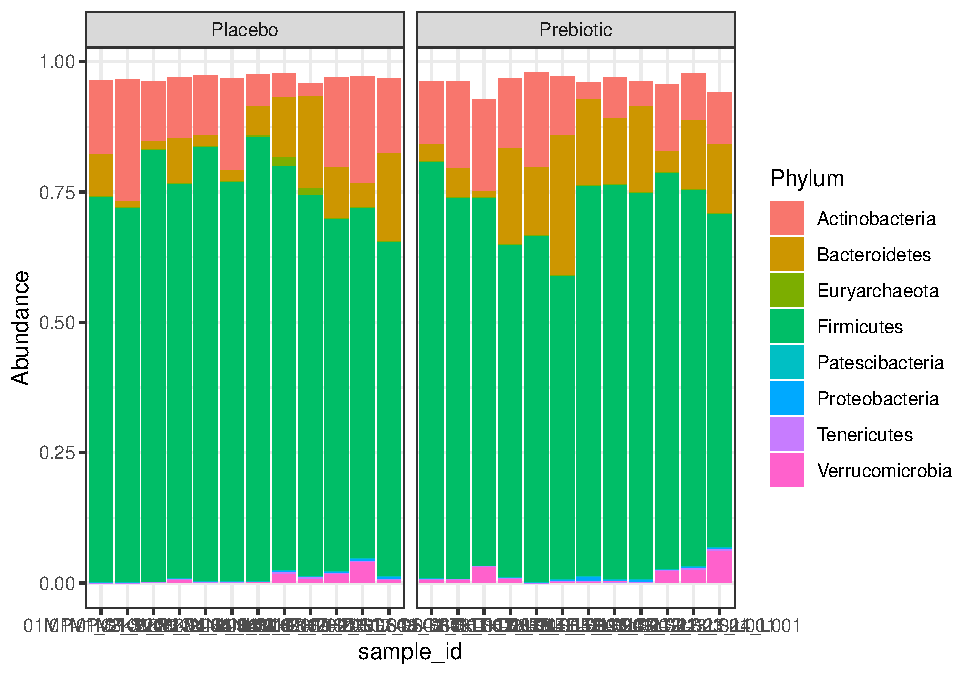
\includegraphics{16sworkshop_files/figure-latex/unnamed-chunk-6-4.pdf}

\begin{Shaded}
\begin{Highlighting}[]
\NormalTok{top10 }\OtherTok{\textless{}{-}} \FunctionTok{names}\NormalTok{(}\FunctionTok{sort}\NormalTok{(}\FunctionTok{taxa\_sums}\NormalTok{(fam), }\ConstantTok{TRUE}\NormalTok{))[}\DecValTok{1}\SpecialCharTok{:}\DecValTok{10}\NormalTok{]}
\NormalTok{fam10 }\OtherTok{\textless{}{-}} \FunctionTok{prune\_taxa}\NormalTok{(top10, fam)}
\NormalTok{fammelt }\OtherTok{\textless{}{-}} \FunctionTok{psmelt}\NormalTok{(fam10)}
\NormalTok{c1 }\OtherTok{\textless{}{-}} \FunctionTok{ggplot}\NormalTok{(fammelt, }\FunctionTok{aes}\NormalTok{(sample\_id, Abundance, }\AttributeTok{fill =}\NormalTok{ Family)) }\SpecialCharTok{+}
  \FunctionTok{geom\_bar}\NormalTok{(}\AttributeTok{stat =} \StringTok{"identity"}\NormalTok{) }\SpecialCharTok{+}
  \FunctionTok{theme\_bw}\NormalTok{() }\SpecialCharTok{+}
  \FunctionTok{facet\_wrap}\NormalTok{(}\SpecialCharTok{\textasciitilde{}}\NormalTok{treatment, }\AttributeTok{scales =} \StringTok{"free\_x"}\NormalTok{)}
\NormalTok{c1}
\end{Highlighting}
\end{Shaded}

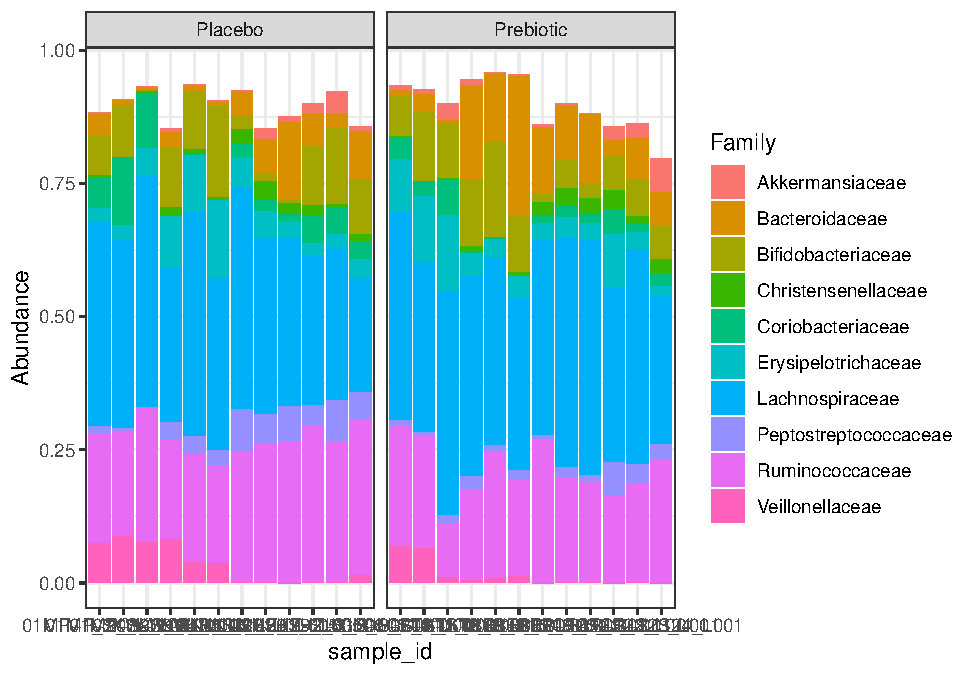
\includegraphics{16sworkshop_files/figure-latex/unnamed-chunk-6-5.pdf}

\begin{Shaded}
\begin{Highlighting}[]
\NormalTok{top10 }\OtherTok{\textless{}{-}} \FunctionTok{names}\NormalTok{(}\FunctionTok{sort}\NormalTok{(}\FunctionTok{taxa\_sums}\NormalTok{(gen), }\ConstantTok{TRUE}\NormalTok{))[}\DecValTok{1}\SpecialCharTok{:}\DecValTok{10}\NormalTok{]}
\NormalTok{gen10 }\OtherTok{\textless{}{-}} \FunctionTok{prune\_taxa}\NormalTok{(top10, gen)}
\NormalTok{genmelt }\OtherTok{\textless{}{-}} \FunctionTok{psmelt}\NormalTok{(gen10)}
\NormalTok{c2 }\OtherTok{\textless{}{-}} \FunctionTok{ggplot}\NormalTok{(genmelt, }\FunctionTok{aes}\NormalTok{(sample\_id, Abundance, }\AttributeTok{fill =}\NormalTok{ Genus)) }\SpecialCharTok{+}
  \FunctionTok{geom\_bar}\NormalTok{(}\AttributeTok{stat =} \StringTok{"identity"}\NormalTok{) }\SpecialCharTok{+}
  \FunctionTok{theme\_bw}\NormalTok{() }\SpecialCharTok{+}
  \FunctionTok{facet\_wrap}\NormalTok{(}\SpecialCharTok{\textasciitilde{}}\NormalTok{treatment, }\AttributeTok{scales =} \StringTok{"free\_x"}\NormalTok{)}
\NormalTok{c2}
\end{Highlighting}
\end{Shaded}

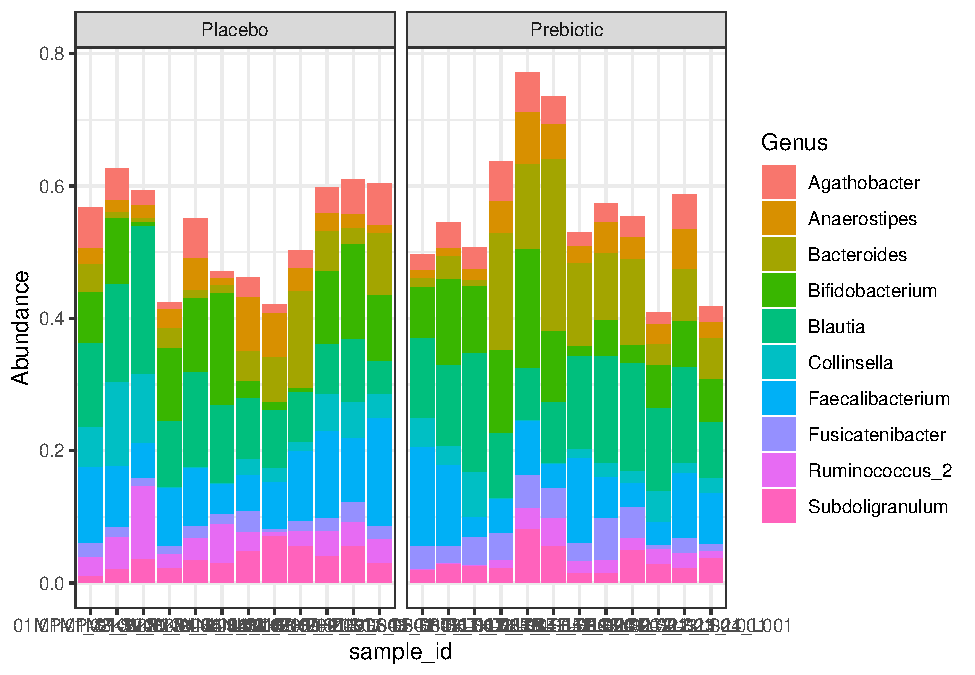
\includegraphics{16sworkshop_files/figure-latex/unnamed-chunk-6-6.pdf}

\hypertarget{what-next}{%
\chapter{What Next?}\label{what-next}}

What you have learnt so far is just the beginging!! There is a lot more ot learn and do.

For example, after looking at beta diversity, you can also look at differential abundance to see which taxa are different in each treatment group or over time.

Most commonly used methods for doing this is \href{https://bioconductor.org/packages/release/bioc/html/DESeq2.html}{deseq2} and a new one is \href{https://github.com/bryandmartin/corncob/}{corncob}. Before using them, please read the papers carefully to know the limitations and correct usage of these pacakages.

Some people also try to do functional analaysis with 16s data and for this \href{https://github.com/picrust/picrust2/wiki}{PICRUST2} pacakge is usually used.

  \bibliography{book.bib,packages.bib}

\end{document}
